% Created 2016-07-07 Thu 07:47
\documentclass[10pt,oneside,x11names]{article}
\usepackage[utf8]{inputenc}
\usepackage[T1]{fontenc}
\usepackage{fixltx2e}
\usepackage{graphicx}
\usepackage{grffile}
\usepackage{longtable}
\usepackage{wrapfig}
\usepackage{rotating}
\usepackage[normalem]{ulem}
\usepackage{amsmath}
\usepackage{textcomp}
\usepackage{amssymb}
\usepackage{capt-of}
\usepackage{hyperref}
\usepackage{geometry}
\usepackage{amsmath}
\usepackage{amssymb}
\usepackage{amsfonts}
\usepackage{palatino}
\usepackage{siunitx}
\usepackage{esdiff}
\usepackage{xfrac}
\usepackage{nicefrac}
\usepackage{faktor}
\usepackage[euler-digits,euler-hat-accent]{eulervm}
\author{Brian Beckman}
\date{\textit{<2016-05-03 Tue>}}
\title{Kalman Folding 5: Non-Linear Models and the EKF (Review Draft)\\\medskip
\large Extracting Models from Data, One Observation at a Time}
\hypersetup{
 pdfauthor={Brian Beckman},
 pdftitle={Kalman Folding 5: Non-Linear Models and the EKF (Review Draft)},
 pdfkeywords={},
 pdfsubject={},
 pdfcreator={Emacs 24.5.1 (Org mode 8.3.4)}, 
 pdflang={English}}
\begin{document}

\maketitle
\setcounter{tocdepth}{2}
\tableofcontents


\section{Abstract}
\label{sec:orgheadline1}

We exhibit a foldable Extended Kalman Filter that internally integrates
non-linear equations of motion with a nested fold of generic
integrators over lazy streams in constant memory.
Functional form allows us to switch integrators easily and to diagnose filter
divergence accurately, achieving orders of magnitude better speed than
the source example from the literature. As with all Kalman folds, we can move
the vetted code verbatim, without even recompilation, from the lab to the field.

\section{Background and Synopsis}
\label{sec:orgheadline2}

In \emph{Kalman Folding, Part 1},\footnote{B. Beckman, \emph{Kalman Folding, Part 1}, \url{http://vixra.org/abs/1606.0328}.} we present basic, static Kalman filtering
as a functional fold, highlighting the unique advantages of this form for
deploying test-hardened code verbatim in harsh, mission-critical environments.

In \emph{Kalman Folding 2: Tracking},\footnote{B. Beckman, \emph{Kalman Folding 2: Tracking and System Dynamics}, \url{http://vixra.org/abs/1606.0348}.} we reproduce a tracking example from
the literature, showing that these advantages extend to linear
models with time-evolving states. 

Here, we extend that example to include aerodynamic drag, making the model
nonlinear. We must change the Kalman filters themselves to handle such problems.
The resulting filters are called \emph{Extended Kalman Filters} or EKFs.

The particular EKF designed here features internal integration of the non-linear
equations of motion. We integrate these equations by folding over a lazy stream
that generates, on demand, differential updates to the solution. Folds over lazy
streams were introduced in \emph{Kalman Folding 4: Streams and Observables},\footnote{B. Beckman, \emph{Kalman Folding 4: Streams and Observables}, to appear.}
where we used them to step a static Kalman filter over observations. Here,
lazy streams afford two advantages:

\begin{enumerate}
\item constant-memory solutions
required for EKFs in embedded systems in the field

\item easy switching of integrators, even at run time, allowing accurate diagnosis and
tuning of the filter
\end{enumerate}

We show these advantages at work by improving Zarchan and Musoff's\footnote{Zarchan and Musoff, \emph{Fundamentals of Kalman Filtering, A Practical
Approach, Fourth Edition}, Ch. 4}
example of tracking the height of a falling object with drag. These authors
exhibit a sequence of filter tunings to converge the filter, ending with a
second-order Runge-Kutta stepped at \(100\) times the observation frequency.
Integration dominates the run-time performance of their example. Because their
integration code is enmeshed with the filter and with data delivery, they were
not easily able to experiment with alternative integrators and missed the
opportunity to try fourth-order Runge-Kutta, which we find converges the filter
\(100\) times faster. 

Other papers in this series feature applications of EKFs to a variety of
problems including navigation and pursuit.

In this series of papers, we use the Wolfram language\footnote{\url{http://reference.wolfram.com/language/}} because it
supports functional programming and it excels
at concise expression of mathematical code. All examples in these papers can be
directly transcribed to any modern mainstream language that supports closures.
For example, it is easy to write them in C++11 and beyond, Python, any modern
Lisp, not to mention Haskell, Scala, Erlang, and OCaml. Many can be written
without full closures; function pointers will suffice, so they are easy to write
in C. It's also not difficult to add extra arguments to simulate just enough
closure-like support in C to write the rest of the examples in that language.

\section{Linear Kalman Accumulator with Time Evolution}
\label{sec:orgheadline4}

In \emph{Kalman Folding 2: Tracking},\footnotemark[2]{} we found the following
accumulator function for a fold that implements the linear
dynamic Kalman filter, that is, a filter that can track states that evolve with
time\footnote{In most applications, the independent variable is physical time,
however, it need not be. For convenience, we use the term \emph{time} to mean \emph{the independent variable of the problem} simply because it is shorter to write.} according to a linear transformation of the state:

\begin{equation}
\label{eqn:kalman-dynamic-cume-definition}
\begin{matrix}
\textrm{kalmanDynamic}
\left(
\left\{
\mathbold{x},
\mathbold{P}
\right\},
\left\{
\mathbold{Z},
\mathbold{\Xi},
\mathbold{\Phi},
\mathbold{\Gamma},
\mathbold{u},
\mathbold{A},
\mathbold{z}
\right\}
\right) = \\
\begin{Bmatrix}
\mathbold{ x }_{ 2 }+
\mathbold{ K }\,
\left(
\mathbold{ z }-
\mathbold{ A }\,
\mathbold{ x }_{ 2 }
\right), &
\mathbold{ P }_{ 2 }-
\mathbold{ K }\,
\mathbold{ D }\,
\mathbold{ K }^\intercal
\end{Bmatrix}
\end{matrix}
\end{equation}

\noindent where

\begin{align}
\label{eqn:state-propagation-equation}
\mathbold{ x }_{ 2 }
&=
\mathbold{ \Phi  }\,
\mathbold{ x }+
\mathbold{ \Gamma  }\,
\mathbold{ u } \\
\label{eqn:covariance-propagation-equation}
\mathbold{ P }_{ 2 }
&=
\mathbold{ \Xi  }+
\mathbold{ \Phi  }\,
\mathbold{ P }\,
\mathbold{ \Phi  }^{ \intercal  } \\
\label{eqn:kalman-gain-definition}
\mathbold{K}
&=
\mathbold{P}\,
\mathbold{A}^\intercal\,
\mathbold{D}^{-1} \\
\label{eqn:kalman-denominator-definition}
\mathbold{D}
&= \mathbold{Z} +
\mathbold{A}\,
\mathbold{P}\,
\mathbold{A}^\intercal
\end{align}

\noindent and all quantities are matrices:

\begin{itemize}
\item \(\mathbold{z}\) is a  \({b}\times{1}\) column vector containing one multidimensional observation
\item \(\mathbold{x}\) and \(\mathbold{x}_{2}\) are \({n}\times{1}\) column vectors of \emph{model states}
\item \(\mathbold{Z}\) is a  \({b}\times{b}\) matrix, the covariance of
observation noise
\item \(\mathbold{P}\) and \(\mathbold{P}_2\) are \({n}\times{n}\) matrices, the theoretical
covariances of \(\mathbold{x}\) and \(\mathbold{x}_2\), respectively
\item \(\mathbold{A}\) is a  \({b}\times{n}\) matrix, the \emph{observation partials}
\item \(\mathbold{D}\) is a  \({b}\times{b}\) matrix, the Kalman denominator
\item \(\mathbold{K}\) is an \({n}\times{b}\) matrix, the Kalman gain
\item \(\mathbold{\Xi}\) is an \(n\times{n}\) integral of \emph{process
noise} \(\mathbold{\xi}\), namely \newline \(\int_{0}^{\delta t}\mathbold{\Phi}(\tau)\cdot{\left(\begin{array}{c|c}\mathbold{0}&\mathbold{0}\\\hline\mathbold{0}&E\left[\mathbold{\xi}\mathbold{\xi}^{\intercal}\right]\end{array}\right)\cdot\mathbold{\Phi}(\tau)^\intercal\,\textrm{d}\tau}\)
\item \(\mathbold{\Phi}\) is the non-dimensional \(n\times{n}\) propagator for \(\mathbold{F}\), namely \(e^{\mathbold{F}\,{\delta t}}\)
\item \(\mathbold{\Gamma}\) is an \(n\times{\dim(\mathbold{u})}\) integral of \emph{system response}, namely \(\int_{0}^{\delta t}{\mathbold{\Phi}(\tau) \cdot \mathbold{G}\,\textrm{d}\tau}\)
\item \(\mathbold{u}\) is a vector of external \emph{disturbances} or \emph{control inputs}
\item \(\delta{t}\) is an increment of time (or, more generally, the independent
variable of the problem)
\end{itemize}

\noindent and the time-evolving states satisfy the following differential
equation in \emph{state-space form}:

\begin{equation}
\label{eqn:state-space-form}
{\dot{\mathbold{x}}}=
\mathbold{F}\,\mathbold{x}+
\mathbold{G}\,\mathbold{u}+
\mathbold{\xi}
\end{equation}

\noindent  \(\mathbold{F}\), \(\mathbold{G}\), and \(\mathbold{u}\) may depend
on time, but not on \(\mathbold{x}\); that is the meaning of ``linear dynamic'' in
this context. 

\subsection{Dimensional Arguments}
\label{sec:orgheadline3}

In physical or engineering applications, these quantities carry physical
dimensions of units of measure in addition to their matrix dimensions as numbers
of rows and columns. Both kinds of dimensions are aspects of the \emph{type} of a
quantity. Dimensional arguments, like type-arguments more generally, are
invaluable for checking equations and code.

If the physical and matrix dimensions of 
\(\mathbold{x}\) 
are
\(\left[\left[\mathbold{x}\right]\right]
\stackrel{\text{\tiny def}}{=}
(\mathcal{X}, n\times{1})\),
of 
\(\mathbold{z}\) 
are
\(\left[\left[\mathbold{z}\right]\right]
\stackrel{\text{\tiny def}}{=}
(\mathcal{Z}, b\times{1})\), 
and of 
\(\delta{t}\)
are
\(\left[\left[\delta{t}\right]\right]
\stackrel{\text{\tiny def}}{=}
(\mathcal{T}, \textrm{scalar})\), 
then

\begin{equation}
\label{eqn:dimensional-breakdown}
\begin{array}{lccccr}
\left[\left[\mathbold{Z}\right]\right]                                       &=& (&\mathcal{Z}^2            & b\times{b}&) \\
\left[\left[\mathbold{A}\right]\right]                                       &=& (&\mathcal{Z}/\mathcal{X}  & b\times{n}&) \\
\left[\left[\mathbold{P}\right]\right]                                       &=& (&\mathcal{X}^2            & n\times{n}&) \\
\left[\left[\mathbold{A}\,\mathbold{P}\,\mathbold{A}^\intercal\right]\right] &=& (&\mathcal{Z}^2            & b\times{b}&) \\
\left[\left[\mathbold{D}\right]\right]                                       &=& (&\mathcal{Z}^2            & b\times{b}&) \\
\left[\left[\mathbold{P}\,\mathbold{A}^\intercal\right]\right]               &=& (&\mathcal{X}\,\mathcal{Z} & n\times{b}&) \\
\left[\left[\mathbold{K}\right]\right]                                       &=& (&\mathcal{X}/\mathcal{Z}  & n\times{b}&) \\
\left[\left[\mathbold{F}\,\mathbold{x}\right]\right]                         &=& (&\mathcal{X}/\mathcal{T}  & n\times{n}&) \\
\left[\left[\mathbold{\Phi}\,\mathbold{x}\right]\right]                      &=& (&\mathcal{X}              & n\times{n}&) \\
\left[\left[\mathbold{G}\,\mathbold{u}\right]\right]                         &=& (&\mathcal{X}/\mathcal{T}  & n\times{1}&) \\
\left[\left[\mathbold{\Gamma}\,\mathbold{u}\right]\right]                    &=& (&\mathcal{X}              & n\times{1}&) \\
\left[\left[\mathbold{\Xi}\right]\right]                                     &=& (&\mathcal{X}^2            & n\times{n}&) \\
\end{array}
\end{equation}

The matrices \(\mathbold{F}\), \(\mathbold{\Phi}\), \(\mathbold{G}\), and
\(\mathbold{\Gamma}\) do not have single dimensions on their own, but their
dimensions in various combinations with other matrices make sense. Elements of
matrix expressions for \(\mathbold{\Xi}\) include sufficient implicit physical
dimensions to make its overall physical dimensions work out to \(\mathcal{X}^2\).
Detailed dimensional analysis of these matrices is the subject of another paper
in this series.

\noindent In all examples in this paper, the observations \(\mathbold{z}\) are
\(1\times{1}\) matrices, equivalent to scalars, so \(b=1\), but the theory and code
carry over to multi-dimensional vector observations.

\section{Tracking with Drag}
\label{sec:orgheadline9}

To accommodate nonlinear equations of state evolution, we replace equation
\ref{eqn:state-propagation-equation} with explicit numerical integration. The
rest of the EKF uses equations \ref{eqn:covariance-propagation-equation},
\ref{eqn:kalman-gain-definition}, and \ref{eqn:kalman-denominator-definition}:
with a propagator \(\mathbold{\Phi}\) derived from first-order linearization.

\subsection{Equations of Motion}
\label{sec:orgheadline5}

Let \(h(t)\) be the height of
the falling object, and let the state vector \(\mathbold{x}(t)\) contain \(h(t)\)
and its first derivative, \(\dot{h}(t)\), the speed of descent.

\begin{equation*}
\mathbold{x} = 
\begin{bmatrix} { h } (t) \\ \dot { h } (t) \end{bmatrix}
\end{equation*}

Omitting, for clarity's sake, explicit dependence of \(h\) and \(\dot{h}\) on time,
the equations of motion are elementary:

\begin{equation}
\label{eqn:equations-of-motion}
\begin{bmatrix} \dot { h } \\ \ddot { h }  \end{bmatrix}
=
\begin{bmatrix}
0 & 1 \\
0 & 0
\end{bmatrix}
\begin{bmatrix} h \\ \dot { h }  \end{bmatrix}
+
\begin{bmatrix} 0 \\ -1 - \textrm{sign}({\dot{h}})\,\rho(h)\,{{\dot{h}}^2}/(2\beta)
\end{bmatrix}
\begin{bmatrix} g \end{bmatrix}
\end{equation}

\noindent where 
\begin{itemize}
\item \(g\) is the acceleration of Earth's gravitation, about
\(32.2\,\textrm{ft}/{\textrm{s}}^2\)
\item \(\rho(h)\) is the density of air in \(\textrm{slug}/{\textrm{ft}}^3\); \(\rho\,{{\dot{h}}^2}\) has
units of pressure, that is, \(\textrm{slug}/(\textrm{ft}\cdot{\textrm{sec}^2})\)
\item \(\beta = 500\,\textrm{slug}/(\textrm{ft}\cdot{\textrm{sec}^2})\)
is a constant \emph{ballistic coefficient}  of the object in units of pressure (it
is possible to estimate this coefficient in the filter; here, we
treat it as a known constant).
\end{itemize}

The positive direction is up and we are only concerned with negative velocities
where the object is approaching the ground. We may provisionally replace the
factor \(\textrm{sign}({\dot{h}})\) with -1 and keep our eye out for improper
positive speeds. 

In scalar form, the equations are 

\begin{equation*}
\ddot { h }
=
g\left(\frac{\rho(h)\,{{\dot{h}}^2}}{2\beta}-1\right)
\end{equation*}

\noindent or 

\begin{equation}
\label{eqn:scalar-equations-of-motion}
\ddot { h }
=
g\left(\frac{A e^{h/k}\,{{\dot{h}}^2}}{2\beta}-1\right)
\end{equation}

\noindent 
with
\(k=22,000\,\left[\textrm{ft}\right]\), the e-folding height of the atmosphere,
and \(A=0.0034\,[\textrm{slug}/{{\textrm{ft}}^3}]\) for the density of
air\footnote{Zarchan and Musoff, on page 228, report \(0.0034\) for the density of air in
\(\textrm{slug}/\textrm{ft}^3\) at the surface; we believe the correct
value is about \(0.00242\) but continue with \(0.0034\) for comparison's sake.} at \(h=0\).

\subsection{Stream Solver}
\label{sec:orgheadline6}

We can write the same differential equation as a lazy stream, which uses only
constant memory. Thus, it is suitable for the internals of a Kalman filter. We
implement the integrator as an accumulator function for \texttt{foldStream} from paper
4 of this series,\footnotemark[3]{} which
produces all intermediate results as a new stream.

The simplest integrator is the Euler integrator, which updates a state with its
derivative times a small interval of time: 

\begin{verbatim}
eulerAccumulator[{t_, x_}, {dt_, t_, Dx_}] :=
  {t + dt, x + dt Dx[x, t]};
\end{verbatim}

Like all accumulator functions, this is a binary function that takes two
arguments. The first is an instance of accumulation type, in this case, a
pair of a scalar time \texttt{t} and a vector state \texttt{x}. The second is an element of
the input stream, a triple of a time differential \texttt{dt}, the same time \texttt{t} that
appears in the first argument, and a function \texttt{Dx} that computes the derivative
of the state given the state and the time as \texttt{Dx[x,t]}.

Folding this integrator over the streamed differential equation produces a
streamed solution. The input stream must produce values of the form 
\texttt{\{dt, t, Dx\}} and, like all streams, also contain a thunk that produces the rest of the
stream.\footnote{Wolfram's ampersand postfix operator can covert its operand into a thunk.}

\begin{verbatim}
dragDStream[Delta : {dt_, t_, Dx_}] :=
  {Delta, dragDStream[{dt, t + dt, Dx}] &};
\end{verbatim}

This \texttt{dragDStream} contains nothing specific to our example, but just increments
time and passes through the integration inputs. It could be much more rich,
manipulating \texttt{dt} and \texttt{Dx} for speed or numerics (\emph{adaptive integration}).

The kernel of our differential equation is the derivative function \texttt{Dx}, which,
for our example, is the following:

\begin{verbatim}
With[{g = 32.2, A = 0.0034, k = 22000., beta = 500.},
  dragD[{x_, v_}, t_] := {v, g (A Exp[-x/k] v^2/(2. beta) - 1)}];
\end{verbatim}

\noindent in which \texttt{x} stands for \(h\) and \texttt{v} for \(\dot{h}\). It is generalized
to handle differential equations that have explicit dependence on a time
variable \texttt{t}, but that parameter is harmlessly ignored in this example.
Integrating the differential equation for thirty seconds looks like this:

\begin{verbatim}
(* constants and initial conditions *)
With[{x0 = 200000., v0 = -6000., t0 = 0., t1 = 30., dt = .1},
 takeUntil[
  foldStream[
   eulerAccumulator,
   {t0, {x0, v0}},
   dragDStream[{dt, t0, dragD}]
   ], First[#] > t1 &]] (* predicate on first elements of solution *)
\end{verbatim}

\begin{figure}[htb]
\centering
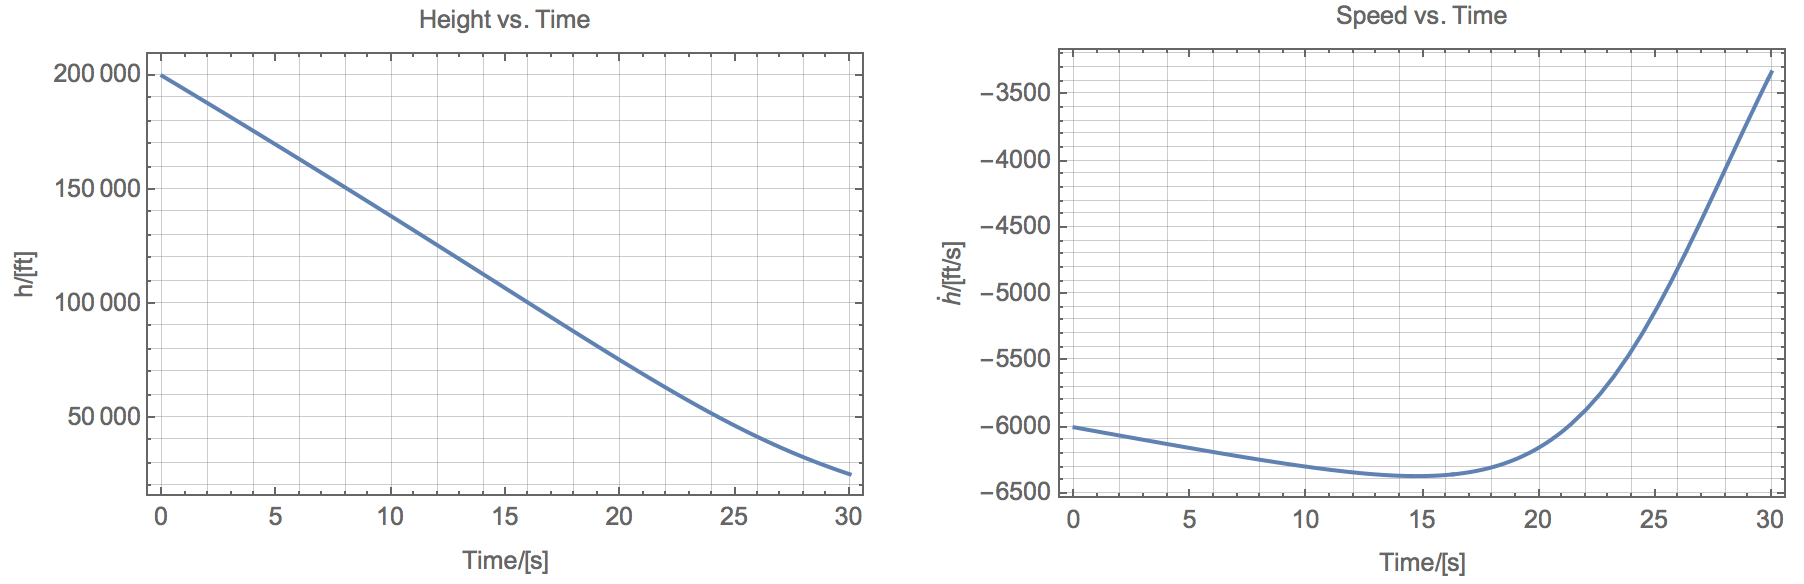
\includegraphics[width=.9\linewidth]{NDSolveFallingWithDrag.png}
\caption{\label{fig:orgparagraph1}
Trajectory of a falling object with drag}
\end{figure}

The type of the result, here, is a lazy stream produced by \texttt{takeUntil} from the
lazy stream produced by \texttt{foldStream}. Because these streams are lazy, nothing
happens until we demand values for, say, plotting, as in figure
\ref{fig:orgparagraph1}. These results are qualitatively
indistinguishable from those in the reference and those produced by Wolfram's
built-in numerical integrator \texttt{NDSolve}, giving us high confidence that we've
got it right.

The arguments of \texttt{takeUntil} are a stream and a predicate, in our case, the
literal function \texttt{First[\#] > t1 \&}. The result is a new
stream that pulls values from the original stream, applying the predicate until
it produces \texttt{True}. 

The implementations of \texttt{foldStream}, \texttt{takeUntil} and other stream operators is
the subject of another paper in this series.

\subsection{What's the Point?}
\label{sec:orgheadline7}

The point of this style of integration is that we can change three aspects of
the integration independently of one another, leaving the others verbatim,
without even recompilation, because we have un-nested and \emph{decomplected}\footnote{``Decomplecting'' is a term coined by Rich Hickey for un-braiding and
un-nesting bits of software.} these aspects:
\begin{enumerate}
\item the integrator
\item potential manipulation of the time increment \texttt{dt} and derivative function \texttt{Dx}
\item the internals of the derivative function \texttt{Dx}
\end{enumerate}

For example, should Euler integration prove inadequate, and it does, we can
easily substitute second- or fourth-order Runge-Kutta integrators. This turns
out to be crucial for a high-performance EKF in this example. The only
requirement on an integrator is that it must match the function signature or
type:

\begin{verbatim}
rk2Accumulator[{t_, x_}, {dt_, t_, Dx_}] :=
  With[{dx1 = dt Dx[x, t]},
   With[{dx2 = dt Dx[x + .5 dx1, t + .5 dt]},
    {t + dt, x + (dx1 + dx2)/2.}]];
rk4Accumulator[{t_, x_}, {dt_, t_, Dx_}] :=
  With[{dx1 = dt Dx[x, t]},
   With[{dx2 = dt Dx[x + .5 dx1, t + .5 dt]},
    With[{dx3 = dt Dx[x + .5 dx2, t + .5 dt]},
     With[{dx4 = dt Dx[x + dx3, t + dt]},
      {t + dt, x + (dx1 + 2. dx2 + 2. dx3 + dx4)/6.}]]]];
\end{verbatim}

Decomplecting these bits also makes them easier to review and verify by hand
because dependencies are lexically obvious, easier
to memorize and to find on a page.

\subsection{Gain and Covariance Updates}
\label{sec:orgheadline8}

For gains and covariances, first-order linear approximations
suffice. If we write the non-linear equations in state-space form as
\(\mathbold{\dot{x}}=f(\mathbold{x})\), then a Taylor series, to first order, yields

\begin{align}
\notag
\mathbold{\dot{x}} &= f(\mathbold{x}_0) + \mathbold{F}(\mathbold{x}_0)\cdot(\mathbold{x}-\mathbold{x}_0) \\
\notag
\Leftrightarrow\mathbold{\dot{x}} &= \mathbold{F}(\mathbold{x}_0)\cdot\mathbold{x} + \mathbold{\dot{x}}_0 - \mathbold{F}(\mathbold{x}_0)\cdot\mathbold{x}_0 
\end{align}

\noindent where \(\mathbold{F}\) is the Jacobian matrix, 

\begin{equation}
\mathbold{F}
\left(
\mathbold{x}=\begin{bmatrix}h\\ \dot{h} \end{bmatrix}
\right) =
\begin{bmatrix}
\underset {  }{ \frac { \partial \dot { h }  }{ \partial h }  }  &
\underset {  }{ \frac { \partial \dot { h }  }{ \partial \dot { h }  }  }  \\
\frac { \partial \ddot { h }  }{ \partial h }  &
\frac { \partial \ddot { h }  }{ \partial \dot { h }  }
\end{bmatrix}
\end{equation}

\noindent and clearly fills the role played by \(\mathbold{F}\) in the linear
state-space form, equation \ref{eqn:state-space-form}. Our linearized
system-dynamics matrix is

\begin{equation}
\mathbold{F}(\mathbold{x}) =
\begin{bmatrix}
\underset {  }{ 0 }  &
\underset {  }{ 1 }  \\
\frac{-A g {\dot{h}}^2 e^{{h}/{k}}}{2 \beta  k}  &
\frac{A g {\dot{h}} e^{{h}/{k}}}{\beta }
\end{bmatrix}
\end{equation}

We need \(\mathbold{\Phi}=e^{\mathbold{F}t}\) to propagate solutions forward,
because, if \(\mathbold{\dot{x}}=\mathbold{F}\,\mathbold{x}\), then
\(e^{\mathbold{F}t}\,\mathbold{x}\)(t) effects a Taylor series. Again, to first
order,

\begin{align}
\notag
\mathbold{x}(t+\delta{t}) &= e^{\mathbold{F}\,\delta{t}}\,\mathbold{x}(t) \\
\label{eqn:expand-f}      &\approx \left(\mathbold{1} + \mathbold{F}\,\delta{t}\right)\,\mathbold{x}(t) \\
\notag                    &= \mathbold{x}(t) + \mathbold{F}\,\mathbold{x}(t)\,\delta{t} \\
\notag                    &\approx \mathbold{x}(t) + \mathbold{\dot{x}}(t)\,\delta{t}
\end{align}

\noindent We take
\(\mathbold{\Phi}(\delta{t})=\mathbold{1}+\mathbold{F}\,\delta{t}\) for our
propagator matrix and  compute the gains and covariances as in equations
\ref{eqn:covariance-propagation-equation}, 
\ref{eqn:kalman-gain-definition}, and
\ref{eqn:kalman-denominator-definition}:

\begin{align}
\mathbold{P}
&\leftarrow
\mathbold{\Xi}+
\mathbold{\Phi}\,
\mathbold{P}\,
\mathbold{\Phi}^\intercal
\end{align}

\noindent where \(\Xi\), integral of the process noise, is 

\begin{equation}
\left(\sigma_\xi\right)^2\cdot
\begin{bmatrix}
 \underset{}{\frac{{\delta t}^3}{3}}
&
 \underset{}{{{{\mathbold{F}_{22}}} {\delta t}^3}/{3}+\frac{{\delta t}^2}{2}}
\\
 {{{\mathbold{F}_{22}}} {\delta t}^3}/{3}+\frac{{\delta t}^2}{2} 
&
 {{{\mathbold{F}_{22}}}^2 {\delta t}^3}/{3}+{{\mathbold{F}_{22}}} {\delta t}^2+{\delta t}
\end{bmatrix}
\end{equation}

\section{The EKF}
\label{sec:orgheadline10}

Though the following code block is bigger than we have seen in earlier papers in
this series, it is a
straight implementation of the notions explained above, highly modularized. The
block of code establishes one global symbol, \texttt{EKFDrag}, which we tune and
analyze in the last section of this paper.

\texttt{With} establishes numerical constants for the equations of motion.
\texttt{Module} establishes local variables to hold the differential-equation kernel and
stream, and for the propagator matrix \(\mathbold{\Phi}\) and process noise
\(\mathbold{\Xi}\). 

\begin{verbatim}
With[{g = 32.2, A = 0.0034, k = 22000., beta = 500.},
 Module[{dragD, dragDStream, F21, F22, Phi, Xi},
\end{verbatim}

The following lines furnish implementations of these functions:

\begin{verbatim}
  (* x stands for h, v for hdot *)
  dragD[{x_, v_}, t_] := {v, g (A Exp[-x/k] v^2/(2. beta) - 1)};
  dragDStream[Delta : {dt_, t_, Dx_}] :=
    {Delta, dragDStream[{dt, t + dt, Dx}] &};
  F21[x_, v_] := -A Exp[-x/k] g v^2/(2. k beta);
  F22[x_, v_] := A Exp[-x/k] g v/beta;
  Phi[dt_, {x_, v_}] := {{1, dt}, {dt*F21[x, v], 1 + dt*F22[x, v]}};
  Xi[dt_, {x_, v_}] := With[{f = F22[x, v]},
    {{dt^3/3, (dt^2*(3 + 2*dt*f))/6}, {(dt^2*(3 + 2*dt*f))/6, 
      dt + dt^2*f + (dt^3*f^2)/3}}];
\end{verbatim}

The EKF itself is in the scope of these variables, and lambda lifts over 
\begin{enumerate}
\item \(\sigma_\xi\), the constant standard deviation of the process noise
\item \(\mathbold{Z}\), the constant observation-noise matrix
\item the integrator function, for instance \texttt{eulerAccumulator} or either of the
Runge-Kutta integrators
\item the filter period \texttt{fdt}
\item the internal integration period \texttt{idt}
\end{enumerate}
allowing independent tuning of all these parameters. Its accumulation type is
\(\{\mathbold{x},\mathbold{P}\}\), as usual. Its observation type includes time
\(t\) because the integrators are all generalized to include it, even though, in
our current example, the differential equations do not depend explicitly on the
time variable. It could be optimized out. The other members of the observation
packet are the usual partials matrix \(\mathbold{A}\) and the observation itself
\(\mathbold{z}\). This is standard Kalman folding as explained in the first paper
in this series.\footnote{B. Beckman, \emph{Kalman Folding, Part 1}, \url{http://vixra.org/abs/1606.0328}.}

The stream operator \texttt{last} forces the lazy integration stream to execute, albeit
in constant memory, until it picks up and returns the final value produced by
\texttt{takeUntil}. This composition of \texttt{last}, \texttt{takeUntil}, and \texttt{foldStream} performs
the EKF's high-precision replacement for the standard Kalman filter's update
equation \ref{eqn:state-propagation-equation}, operating at the integration
period \texttt{idt}. The rest of the code implements equations
\ref{eqn:covariance-propagation-equation}, \ref{eqn:kalman-gain-definition}, and
\ref{eqn:kalman-denominator-definition} with the linearized propagator \texttt{Phi}
operating at the filter period \texttt{fdt}.

\begin{verbatim}
EKFDrag[sigmaXi_, Zeta_, integrator_, fdt_, idt_]
  [{x_, P_}, {t_, A_, z_}] :=
  Module[{x2, P2, D, K},
   x2 = last[takeUntil[foldStream[integrator, {t, x},
        dragDStream[{idt, t, dragD}]],
       First@# > t + fdt &]][[2]];
   P2 = sigmaXi^2 Xi[fdt, x] + Phi[fdt, x].P.Transpose[Phi[fdt, x]];
   D = Zeta + A.P2.Transpose[A];
   K = P2.Transpose[A].inv[D];
   {x2 + K.(z - A.x2), P2 - K.D.Transpose[K]}];
\end{verbatim}

\section{Tuning and Performance}
\label{sec:orgheadline11}

Because we can tune five parameters of the filter independently, we can efficiently
explore the tuning space. The first task is to reproduce the author's results,
then to look for opportunities to improve them.

\begin{figure}[htb]
\centering
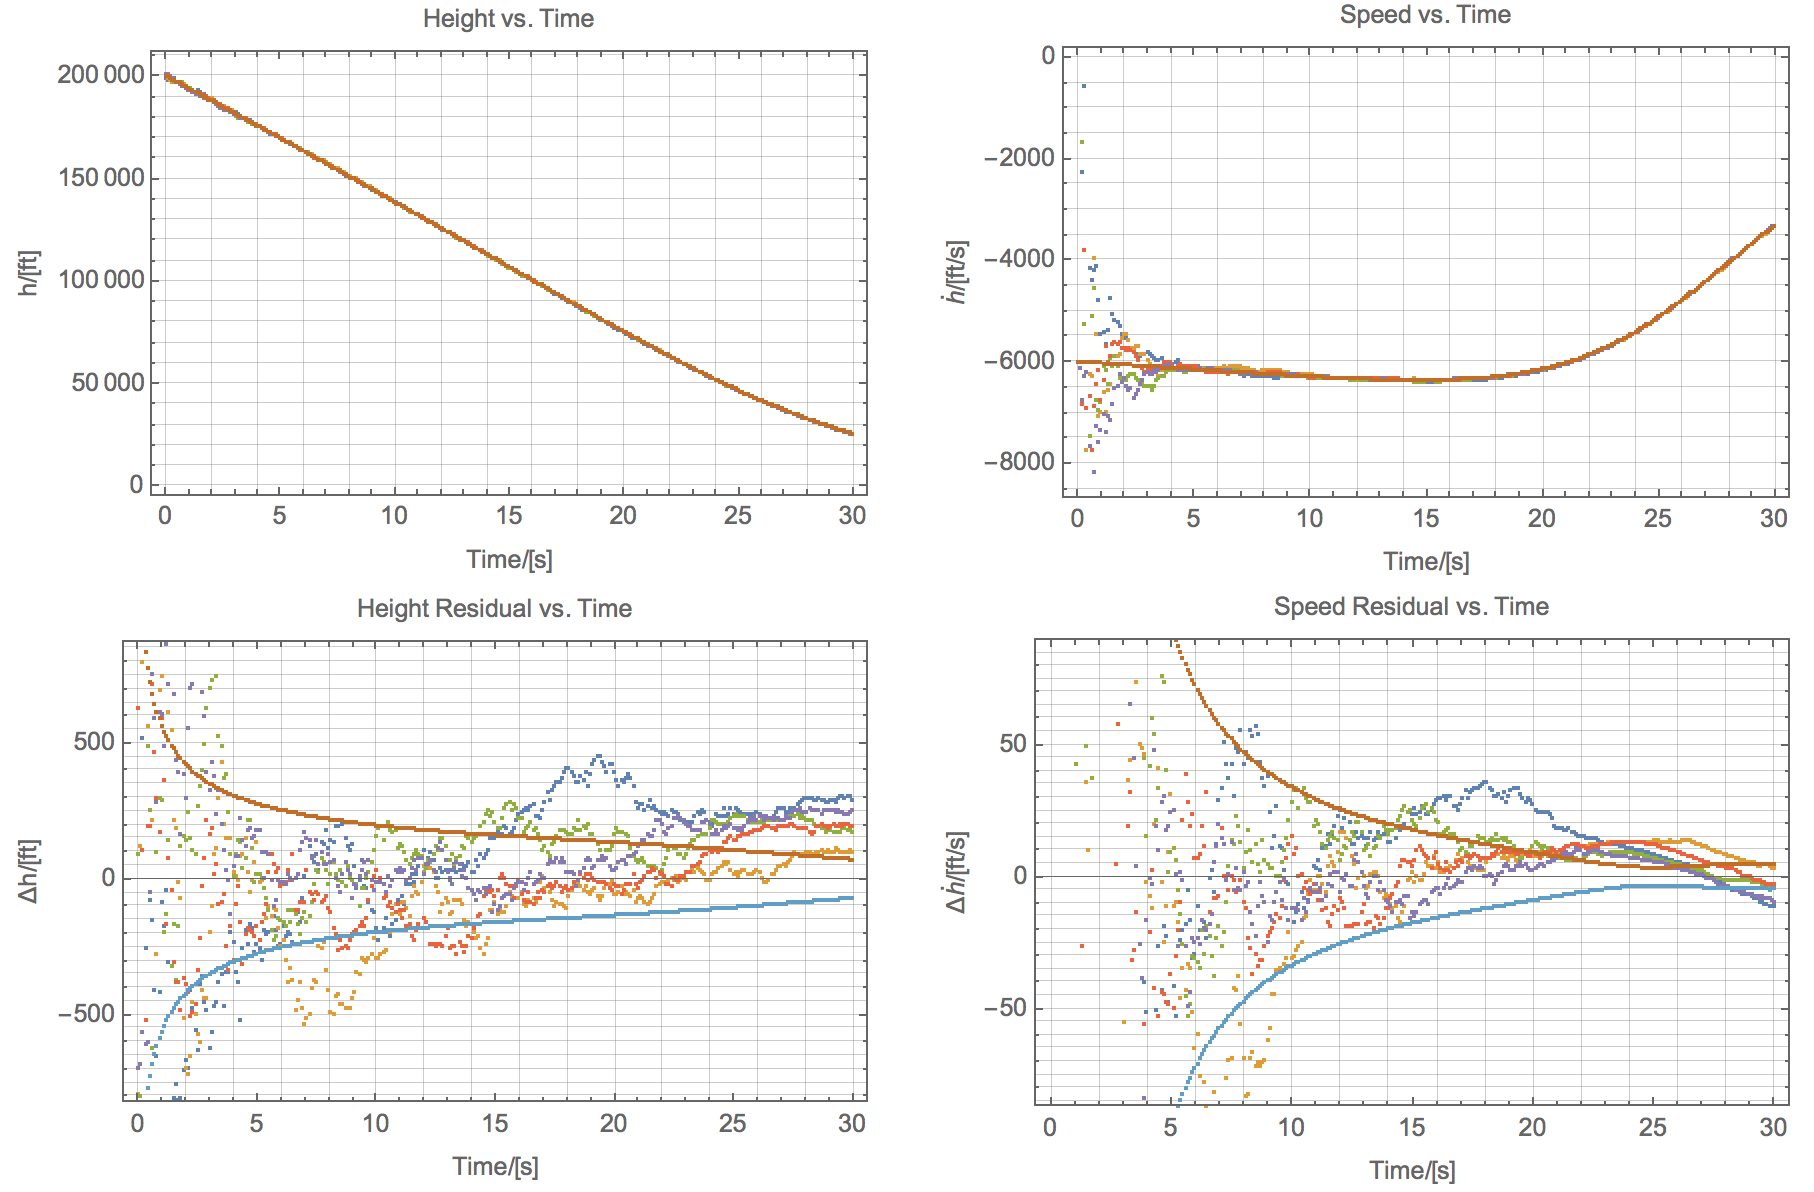
\includegraphics[width=.9\linewidth]{euler-idt-point-1-zeta-1000.png}
\caption{\label{fig:orgparagraph2}
Euler integrator, \texttt{idt} \(= 0.1\) sec, \(\sigma_\zeta = 1000\) ft}
\end{figure}

Zarchan and Musoff report filter convergence and excellent speed for the Euler
integrator operating at a period of \(0.1\) seconds, exactly the same as the
filter period, and a standard deviation of \(1,000\,\textrm{ft}\) for observation
noise. We reproduce their results qualitatively in figure
\ref{fig:orgparagraph2}, by folding \texttt{EKFDrag} over a lazy stream of
deterministically pseudorandom observations. The smoother lines represent
one-sigma theoretical covariance envelopes and the noisy dots represent five
iterations of the filter over faked data.

Figure \ref{fig:orgparagraph2} exhibits overall convergence, but there
are signs of trouble for times beyond \(20\) sec. These are visually obvious, but
would be difficult to detect statistically. 

\begin{figure}[htb]
\centering
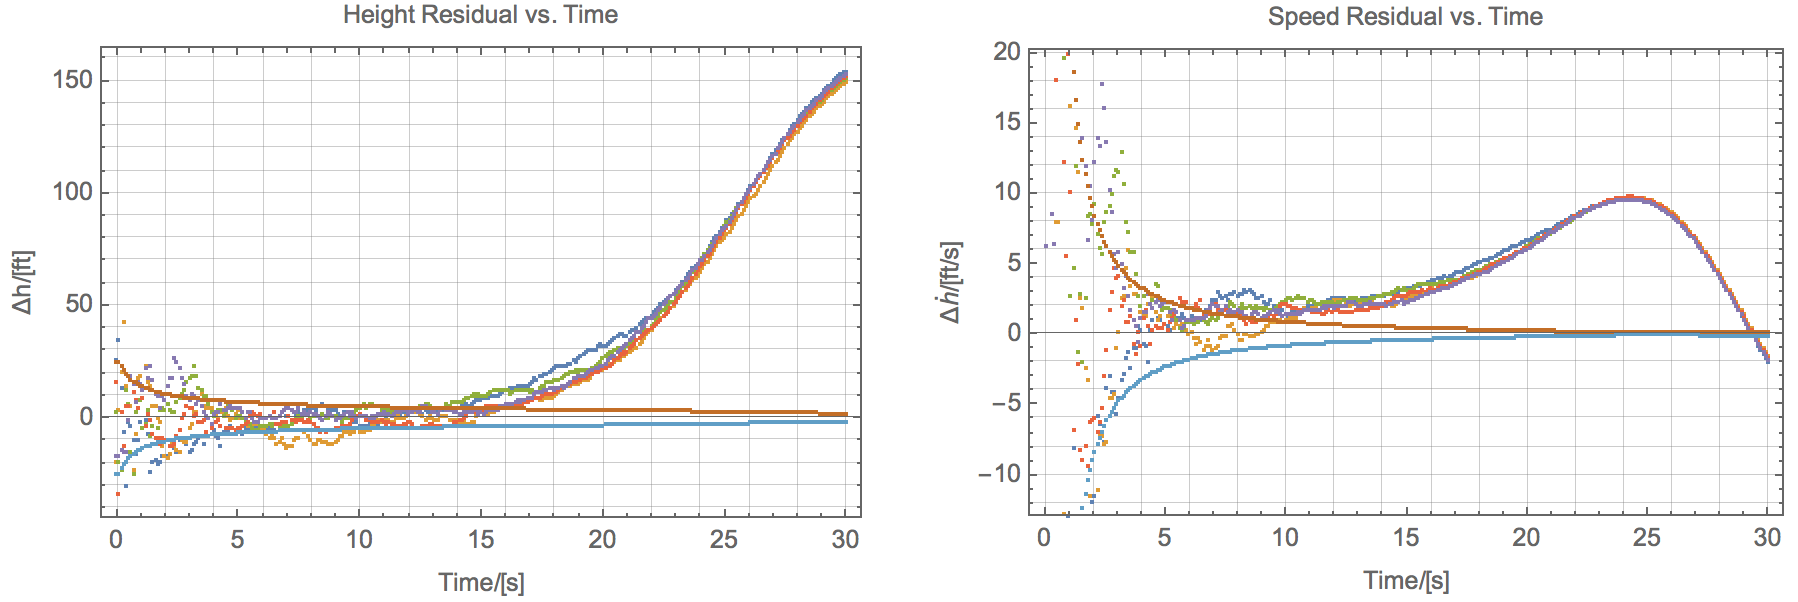
\includegraphics[width=.9\linewidth]{euler-idt-point-1-zeta-25.png}
\caption{\label{fig:orgparagraph3}
Euler integrator, \texttt{idt} \(= 0.1\) sec, \(\sigma_\zeta = 25\) ft}
\end{figure}

\begin{figure}[htb]
\centering
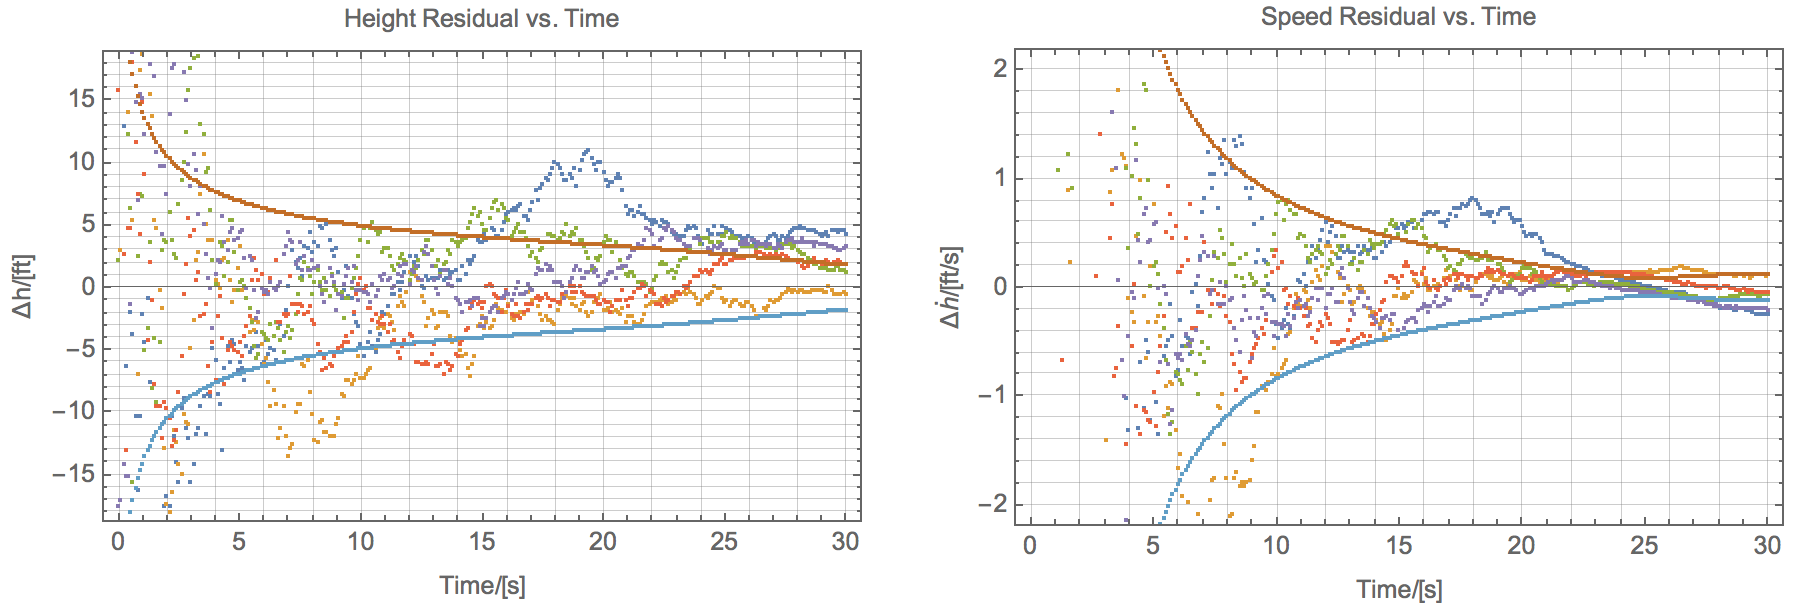
\includegraphics[width=.9\linewidth]{rk2-idt-point-001-zeta-25.png}
\caption{\label{fig:orgparagraph4}
RK-2 integrator, \texttt{idt} \(= 0.001\) sec, \(\sigma_\zeta = 25\) ft; also RK-4 integrator, \texttt{idt} \(= 0.1\) sec}
\end{figure}

The authors report, and we concur, complete filter failure when the observation
standard deviation is reduced to \(25\) feet, which forces the filter to rely much
more on the integrator than on the observations at higher times because it has
been told that the observations are reliable (low sigma). This interpretation is
confirmed by the squeezing of the covariance envelopes in figure
\ref{fig:orgparagraph3}. The filter slavishly follows the integrator and
seems to accumulate its floating-point errors into bad estimates. A detailed
numerical analysis of this phenomenon is beyond the scope of this paper, but the
authors gain evidence that this is the case, and we concur, by moving to a
second-order Runge-Kutta integrator. They find, and we concur, that they must
move to an integration period of \(0.001\) seconds, \(100\) times slower, to regain
convergence. See figure \ref{fig:orgparagraph4}.

We were able to restore the speed of the filter and produce results visually
indistinguishable from figure \ref{fig:orgparagraph4} with the
fourth-order Runge-Kutta integrator simply by feeding those parameters into
\texttt{EKFDrag}. Now suitably tuned, the filter can be deployed verbatim, without even
recompilation, in the field. We emphasize the importance of verbatim deployment,
as in the first paper in this series, because floating-point issues are
extremely sensitive to the slightest change. We have seen many cases where even
changing the order of operations by compiler optimizer flags or by targeting
different versions of the same processor family produce qualitatively different
results due to non-associativity of floating point math and accumulation
phenomena. 

We note in passing that Zarchan and Musoff also find, and we concur, that
increasing the order of the Taylor series for computing \(\mathbold{\Phi}\) and
\(\mathbold{\Xi}\) does not qualitatively improve the filter. That option might
become relevant and important at longer filter periods \texttt{fdt} or in other
applications.

\section{Concluding Remarks}
\label{sec:orgheadline12}

The Extended Kalman Filter (EKF) typically handles non-linear problems by propagating
states with high-precision integration and propagating 
Kalman gain and state covariance by linear approximations. The benefits of
writing EKFs as folds over lazy streams include high modularity, allowing
efficient and accurate tuning and diagnosis, and the flexibility to deploy
fragile floating-point code verbatim, without even recompilation, from the lab
to the field.
\end{document}